% !TEX TS-program = pdflatex
% !TEX encoding = UTF-8 Unicode

% This is a simple template for a LaTeX document using the "article" class.
% See "book", "report", "letter" for other types of document.

\documentclass[20pt]{article} % use larger type; default would be 10pt

\usepackage[utf8]{inputenc} % set input encoding (not needed with XeLaTeX)

%%% Examples of Article customizations
% These packages are optional, depending whether you want the features they provide.
% See the LaTeX Companion or other references for full information.

%%% PAGE DIMENSIONS
\usepackage{geometry} % to change the page dimensions
\geometry{a4paper} % or letterpaper (US) or a5paper or....
% \geometry{margin=2in} % for example, change the margins to 2 inches all round
% \geometry{landscape} % set up the page for landscape
%   read geometry.pdf for detailed page layout information
\usepackage{titlesec}
\usepackage{graphicx} % support the \includegraphics command and options

% \usepackage[parfill]{parskip} % Activate to begin paragraphs with an empty line rather than an indent

%%% PACKAGES
\usepackage{booktabs} % for much better looking tables
\usepackage{array} % for better arrays (eg matrices) in maths
\usepackage{paralist} % very flexible & customisable lists (eg. enumerate/itemize, etc.)
\usepackage{verbatim} % adds environment for commenting out blocks of text & for better verbatim
%\usepackage{subfig} % make it possible to include more than one captioned figure/table in a single float
\usepackage{mathtools}
\usepackage{graphicx} % supports images in latex
% These packages are all incorporated in the memoir class to one degree or another...

\usepackage{graphicx}
\usepackage{subcaption}

%%% Other stuff
\DeclarePairedDelimiter\ceil{\lceil}{\rceil}
\DeclarePairedDelimiter\floor{\lfloor}{\rfloor}

%%% HEADERS & FOOTERS
\usepackage{fancyhdr} % This should be set AFTER setting up the page geometry
\pagestyle{fancy} % options: empty , plain , fancy
\renewcommand{\headrulewidth}{0pt} % customise the layout...
\lhead{}\chead{}\rhead{}
\lfoot{}\cfoot{\thepage}\rfoot{}

%%% SECTION TITLE APPEARANCE
\usepackage{sectsty}
\allsectionsfont{\sffamily\mdseries\upshape} % (See the fntguide.pdf for font help)
% (This matches ConTeXt defaults)

%%% ToC (table of contents) APPEARANCE
\usepackage[nottoc,notlof,notlot]{tocbibind} % Put the bibliography in the ToC
\usepackage[titles,subfigure]{tocloft} % Alter the style of the Table of Contents
\renewcommand{\cftsecfont}{\rmfamily\mdseries\upshape}
\renewcommand{\cftsecpagefont}{\rmfamily\mdseries\upshape} % No bold!

%%% graphics path

\usepackage{listings}
%\begin{lstlisting}[language=java]
%\end{lstlisting}

%%% END Article customizations

%%% nice things to keep around
%\begin{figure}[!htbp]
%  	\centering
%   	\begin{subfigure}[p]{0.5\linewidth}
%    	\includegraphics[width=\linewidth]{}
%   	\end{subfigure}
%\end{figure} 

% \noindent\rule{2cm}{0.4pt} 
%%% puts a small horizontal line

% \mathcal{O} 
%%% big O notation

% \begin{table}[!htbp]
% \caption{Forward slash.}
% \[\begin{array}{c|ccccc} 
% abc/def & 1 & 2 & 3 & 4 & 5\\
% \hline
% 1 & a & b & c & d & e\\
% 2 & f & g & h & i & j\\
% 3 & k & l & m & n & o\\
% \end{array}\]
% \end{table}

%%% The "real" document content comes below...

\title{Formal Languages Final Study guide}
\author{Liam Dillingham}
%\date{} % Activate to display a given date or no date (if empty),
         % otherwise the current date is printed 

\begin{document}
\maketitle

\section{Definitions}
\subsection{Strings}
\begin{itemize}
\item $\Sigma$: alphabet.  An alphabet is a \textit{finite} set of symbols (not including $\epsilon$)
\item $\Sigma^{k}$: strings from the alphabet $\Sigma$ of length $k$
\item $\Sigma^{*}$: The set of all strings over an alphabet (including $\Sigma^{0}$ i.e. $\epsilon$).
\item $\Sigma^{+}$: set of non-empty strings
\item A language $L$ is a set of strings from the alphabet $\Sigma^{*}$ such that $L \subseteq \Sigma^{*}$
\end{itemize}
\subsection{Finite Automata}
\subsubsection{Deterministic Finite Automata}
A \textit{DFA}, labeled as $A$, is defined as $A = (Q, \Sigma, \delta, q_0, F)$, such that:
\begin{enumerate}
\item $Q$: a finite set of \textit{states}
\item $\Sigma$: a finite set of \textit{input symbols}
\item $\delta(q, a)$: a transition function with arguments as $q$: the current state, and $a$: the current input symbol, where $\delta: Q \times \Sigma \rightarrow Q$
\item $q_0$, or the starting state in $Q$
\item $F$: The set of final or accepting states such that $F \subseteq Q$.
\end{enumerate}
\paragraph{Extended Transition Function}  $\hat{\delta}(q,w) = \delta(\hat{\delta}(q,x), a)$\\
The \textit{extended transition function} precisely describes what happens when we start in any state and follow any sequence of inputs i.e. defines $\delta$ for whole words instead of symbols
\paragraph{Language of DFA} if $A$ is a DFA, then $L(A) = \{ w \mid w \in \Sigma^{*}$ and $\hat{\delta}(q_0, w) \in F \}$
\subsubsection{Nondeterministic Finite Automata}
The only difference between a \textit{DFA} and \textit{NFA} is that for an \textit{NFA}, $\delta$ maps to a set of states. that is, $\delta: Q \times \Sigma \rightarrow 2^{Q}$ i.e. $\mathcal{P}(Q)$
\paragraph{Extended Transition Function}
$$\text{basis: } \hat{\delta}(q, \epsilon) = q. \text{  induction: } \hat{\delta}(q,w) = \hat{\delta}(q, xa) = \bigcup_{p \in \hat{\delta}(q,x)}\delta(p,a)$$
\subsubsection{$\epsilon$-Nondeterministic Finite Automata}
For $\epsilon$\textit{-NFA}, we explicitly define transitions for $\epsilon$, i.e. $\delta: Q \times (\Sigma \cup \{ \epsilon \}) \rightarrow 2^{Q}$
\paragraph{Extended Transition Function}
\begin{itemize}
\item \textbf{ECLOSE($q$)}: All the states that $q$ can reach using only $\epsilon$
\item \textbf{ECLOSE($S$)}: $\bigcup_{r \in S}$ \textbf{ECLOSE($r$)}, where $S$ is a set of states
\end{itemize}
For the precise definition, we have: 
$$\text{basis: } \hat{\delta}(q, \epsilon) = \text{\textbf{ECLOSE($q$)}. } \ \hat{\delta}(q,w) = \hat{\delta}(q, xa) = \text{\textbf{ECLOSE}} \Bigg( \bigcup_{p \in \hat{\delta}(q,x)}\delta(p,a) \Bigg)$$
The language described by an $\epsilon$\textit{-NFA}, $A$, is defined as: $A = \{ w \mid \hat{\delta}(q_0, w) \cap F \neq \emptyset \}$.
\subsubsection{Equivalence of States}
We say two states $p,q$, are \textit{equivalent}, if, for all input strings $w$, $\hat{\delta}(p,w)$ is an accepting state if and only if $\hat{\delta}(q,w)$ is an accepting state. That is: \\
$q \equiv p \Leftrightarrow \forall w \in \Sigma^{*}, \hat{\delta}(q,w), \hat{\delta}(p,w) \in F$ or $\hat{\delta}(p,w) \notin F$
\subsection{Properties of Regular Languages}
\subsubsection{The Pumping Lemma}
\paragraph{The pumping lemma for regular languages}  Let $L$ be a regular language. Then there exists a constant $n$ (which depends on $L$) such that for every string $w$ in $L$ such that $|w| \geq n$, we can break $w$ into three strings, $w = xyz$ such that:
\begin{enumerate}
\item $y \neq \epsilon$
\item $|xy| \leq n$
\item For all $k \geq 0$, the string $xy^{k}z$ is also in $L$
\end{enumerate}
That is, we can always find  a nonempty strings $y$ not too far from the beginning of $w$ that can be "pumped"; that is, repeating $y$ any number of times, or deleting it (case $k=0$), keeps the string in the language $L$.  If the string stays in the language $L$, then $L$ is \textbf{regular}.
\newpage
\subsection{Grammars}
\subsubsection{General Grammar Defintion}
\paragraph{$G = (V, T, P, S)$}
\begin{itemize}
\item $V$: finite set of \textit{variables} or \textit{nonterminals}
\item $T$: finite set of terminals $V \cap T = \emptyset$
\item $P$: finite set of \textit{productions} or \textit{rules} of the form $\alpha \rightarrow \beta$ are strings and what symbols a string may contain differentiates different types of grammars to be defined later
\item $S$: the \textit{start symbol}
\end{itemize}
\subsubsection{Derivations}
\paragraph{Relating two strings by a \textit{production} or rule "$\Rightarrow$"}
\begin{itemize}
\item Let $\alpha \rightarrow \beta$ be a rule, we have:
\item $x\alpha y \Rightarrow x\beta y$, where $x,y \in (V \cup T)^{*}$
\end{itemize}
\paragraph{Left-most Derivations:} At each step we replace the leftmost varaible by one of its production bodies
\paragraph{Right-most Derivations:} At each step we replace the rightmost varaible by one of its production bodies
\paragraph{Relating two string by a sequence of productions or rules "$\Rightarrow^{*}$"}
\begin{itemize}
\item Let $w_0 \Rightarrow w_1, w_1 \Rightarrow w_2, ..., w_{k-1} \Rightarrow w_k$
\item $w_0 \Rightarrow^{*} w_k$ where $w_i \in (V \cup T)^{*}$
\end{itemize}
\subsubsection{Sentential Form}
\begin{itemize}
\item if $S \Rightarrow^{*} \alpha, \alpha \in (V \cup T)^{*}$, then $\alpha$ is called a \textit{sentential form}
\item Sentence: if $S \Rightarrow^{*} \alpha, \alpha \in T^{*}$, then $\alpha$ is called a \textit{sentence}
\item The language generated by grammar: $G = (V, T, P, S)$, where $L = \{ w \mid S \Rightarrow^{*} w, w \in T^{*} \}$, or the set of all sentences.
\end{itemize}
\subsubsection{Parse Trees}
Given a grammar $G = (V, T, P, S)$. The \textit{parse trees} for $G$ are trees with the following conditions:
\begin{enumerate}
\item Each interior node is labeled by a variable in $V$.
\item Each leaf is labeled by either a variable, a terminal, or $\epsilon$. However, if the leaf is labeled $\epsilon$, then it must be the only child of its parent.
\end{enumerate}
\subsubsection{Definition: \textbf{Context-Free Grammar}}
$G = (V, T, P, S)$
\begin{itemize}
\item $V$: finite set of \textit{variables} or \textit{nonterminals}
\item $T$: finite set of terminals $V \cap T = \emptyset$
\item $P$: a finite set of production rules of the form $\alpha \rightarrow \beta$, where $\alpha \in V$, and $\beta \in (T \cup V)^{*}$
\item $S$: the \textit{start symbol}
\end{itemize}
\subsubsection{Definition: \textbf{Regular Grammar}}
$G = (V, T, P, S)$
\begin{itemize}
\item $V$: finite set of \textit{variables} or \textit{nonterminals}
\item $T$: finite set of terminals $V \cap T = \emptyset$
\item $P$: a finite set of production rules of the form $\alpha \rightarrow \beta$, where $\alpha \in V$, and $\beta \in (T \cup TV \cup \{ \epsilon \})$
\item $S$: the \textit{start symbol}
\end{itemize}
\subsubsection{Definition: \textbf{Context-Sensitive Grammar}}
$G = (V, T, P, S)$
\begin{itemize}
\item $V$: finite set of \textit{variables} or \textit{nonterminals}
\item $T$: finite set of terminals $V \cap T = \emptyset$
\item $P$: a finite set of production rules of the form $\alpha \rightarrow \beta$, where $\alpha \in (V \cup T)^{+}$, and $\beta \in (T \cup V)^{*}$, and $|\alpha| \leq |\beta|$.
\item $S$: the \textit{start symbol}
\end{itemize}
\subsubsection{Definition: \textbf{Unrestricted Grammar}}
$G = (V, T, P, S)$
\begin{itemize}
\item $V$: finite set of \textit{variables} or \textit{nonterminals}
\item $T$: finite set of terminals $V \cap T = \emptyset$
\item $P$: a finite set of production rules of the form $\alpha \rightarrow \beta$, where $\alpha \in (V \cup T)^{+}$, and $\beta \in (T \cup V)^{+}$.
\item $S$: the \textit{start symbol}
\end{itemize}
\subsubsection{Ambiguous Grammars}
For some CFG's, it is possible to find a terminal string with more than one parse tree, or equivalently, more than one most left-most derivation.
\subsection{Pushdown Automata}
\subsubsection{Non-deterministic PDA}
$P = (Q, \Sigma, \Gamma, \delta, q_0, Z_0, F)$
\begin{itemize}
\item $\Gamma$: Finite set of \textit{stack symbols}
\item $Z_0$: initial \textit{Top of stack} (can be removed)
\item $\delta: Q \times (\Sigma \cup \{ \epsilon \}) \times \Gamma \rightarrow 2^{Q \times \Gamma^{*}}$ or rather, $Q \times \Gamma^{*} = \{ (q,\gamma) \mid q \in Q, \gamma \in \Gamma^{*} \}$
\end{itemize}
\paragraph{Instantaneous Description of PDA: } $($\textbf{current state}, \textbf{next input}, \textbf{top of stack}$) \vdash ($\textbf{next state}, \textbf{next input}, \textbf{next top}$)$
\paragraph{Language Accepted by \textbf{Final State}: } $L = \{ w \mid (q,w, Z_0) \vdash^{*} (p \epsilon, \gamma)$, where $p \in F$, and $\gamma \in \Gamma^{*} \}$
\paragraph{Language Accepted by \textbf{Empty Stack}: } $L = \{ w \mid (q_0, w Z_0) \vdash^{*} (p, \epsilon, \epsilon), p \in Q \}$
\subsubsection{Deterministic PDA (DPDA)}
\begin{enumerate}
\item $\delta(q, a, z)$: contains single Entry $a \in \Sigma \cup \{ \epsilon \}, z \in \Gamma$
\item if $delta(q, \epsilon, z)$ is defined, then $\delta(q, a, z)$ is empty, for ($a \in \Sigma, z \in \Gamma$).
\end{enumerate}
\subsection{Context-Free Language Pumping Lemma}
Let $L$ be a CFL. Then there exitsts a constant $n$ such that if $z$ is any string in $L$ such that $|z|$ is at least $n$, then we can write $z = uvwxy$, subject to the following conditions:
\begin{enumerate}
\item $|vwx| \leq n$. That is, the middle portion is not too long.
\item $vx \neq \epsilon$. Since $v$ and $x$ are the pieces to be "pumped", this condition says that at least one of the strings we pump must not be empty
\item For all $i \geq 0$, $uv^{i}wx^{i}y$ is in $L$. That is, the two strings $v$ and $x$ may be "pumped" any number of times, including 0, and the resulting string will still be a member of $L$. 
\end{enumerate}
\subsection{Chomsky Normal Form for CFG}
\subsubsection{\textbf{Chomsky Normal Form} Algorithm to transform into CNF:}
\begin{itemize}
\item Eliminate \underline{$\epsilon$-productions}
\item Eliminate \underline{unit productions}
\item Eliminate \underline{useless} symbols, i.e., Variables which \textbf{do not} generate \underline{terminals} or are \textbf{not} reachable from $S$
\end{itemize}
\subsubsection{Nullable Computation}
\begin{itemize}
\item $N_0 = \{ A \mid A \rightarrow \epsilon \}$ (basis)
\item $N_1 = \{ A \mid A \rightarrow \alpha, \alpha \in N_0^{*} \} \cup N_0$ (induction)
\item When $N_k = N_{k+1}. N_k$ is the set of \underline{all} nullable
\end{itemize}
\begin{enumerate}
\item Eliminate $A \rightarrow \epsilon$
\item Introduce new rules for every combination of \underline{nullable} to \underline{$\epsilon$}
\item repeat $(1)$ and $(2)$ for each rule
\end{enumerate}
\subsubsection{Unit Computation}
When there is no $\epsilon$-production:
\begin{itemize}
\item $unit(A) = \{ B \mid A \Rightarrow^{*} B \}$
\item $u_0(A) = \{A\}$
\item $u_1(A) = \{B \mid A \Rightarrow B \} \cup u_0(A)$
\end{itemize}
When $u_k(A) = u_{k+1}(A), u_k(A)$ is the set of variables $A$ can reach via production
\begin{enumerate}
\item Eliminate all unit production
\item Promote $B \rightarrow w$ to $A$ for each $B \in u_k(A)$
\end{enumerate}
\subsubsection{Generating Computation}
\begin{itemize}
\item $G_0 = \{ A\mid A \rightarrow w, w \in T^{*}\}$
\item $G_1 = \{A \mid A \rightarrow w, w \in (T \cup G_0)^{*} \} \cup G_0$
\end{itemize}
When $G_k = G_{k+1}, G_k$ is the set of all variables that is generating.  Get rid of variables or rules that involve not generating Variables
\subsubsection{Reachable from $S$ Computation}
\begin{itemize}
\item $S_0 = \{S\}$
\item $S_1 = \{ A \mid B \rightarrow \alpha A B, B \in S_0, \alpha, \beta \in (V \cup T)^{*} \} \cup S_0$
\end{itemize}
When $S_k = S_{k+1}, S_k$ is the set of variables reachable from $S$.
\subsection{Church-Turing Thesis}
"The unprovable assumption that any general way to compute will allow us to compute only the partial-recursive functions (or equivalently, what Turing machines or modern-day computers can compute) is known as \textit{Church's hypothesis}\\
The \textit{Church Turing Thesis} shows that if a TM always halts then it is a rec. lang.  If it only halts on accept then it is rec. enum.  (tentative)
\subsection{Turing machines}
\subsubsection{Definition of Turing machine}
\begin{itemize}
\item $M = (Q, \Sigma, \Gamma, \delta, q_0, B, F)$.
\item $\delta: Q \times \Gamma \rightarrow Q \times \Gamma \times \{ L, R \}$, where $\delta(q,a) = (P, b, \overset{L}{R})$
\end{itemize}
\subsubsection{Languages of Turing Machines}
$L = \{ q_0 w \vdash^{*} \alpha_1q_f\alpha_2, \ \alpha_1, \alpha_2 \in \Gamma^{*}, \ q_f \in F \}$
\paragraph{Closure of Languages: } regular $\subset$ CFL $\subset$ CSL $\subset$ recursive $\subset$ rec. enum. $\subset$ non-rec. enum
\paragraph{Recursive and Recursively Enumerable Languages} A language which accepts on halting
\subsection{Diagonalization Language ($L_d$)}
The language $L_d$ the \textit{diagonalization language}, is the set of strings $w_i$ such that $w_i$ is not in $L(M_i)$.  That is, $L_d = \{ w_i \mid w_i \notin L(M_i)$ where $w_i = \textless M_i \textgreater \}$.  Note that $L_d$ is not recursively enumerable.
\subsection{Universal Language ($L_u$)}
$L_u = \{ (M, w) \mid w \in L(M)\}$ Where $M$ is a TM of the binary alphabet which accepts $w$. $U$ is a \textit{universal} TM such that: $L(U) = \{ (M,w) \mid \textless M \textgreater 111 w$ is accepted by $U \}$, and $L(U) = L_u$.
\subsection{$L_e$ and $L_{ne}$}
dont' know yet
\subsection{Decidable or Undecidable Problems}
A preview of \textbf{Undecidable CFL} problems:
\begin{enumerate}
\item is a given CFG $G$ ambiguous?
\item is a given CFL inherently ambiguous?
\item is the intersection of two CFL's empty?
\item are two CFL's the same?
\item is a given CFL equal to $\Sigma^{*}$, where $\Sigma$ is the alphabet of this language?
\end{enumerate}
\subsection{The Halting Problem}
The halting problem is an issue of decidability
\subsection{Halting Language ($L_H$)}
$L_H$ is the set of languages which halt.  this is why the halting problem is recursively enumerable, because the language itselfs is TMs which halt on their own encoding.  since a rec. enum. language always halts on accept, and the language is the set of TM's who halt on their own encoding, then $L_H$ is rec. enum.

\newpage
\section{Algorithms}
\subsection{\textit{reduce} DFA states (e.g. convert to \textbf{regular expression}}
Remember to add $^{*}$ to loops.  Union multiple loops with $+$
\begin{figure}[!htbp]
  	\centering
   	\begin{subfigure}[p]{0.5\linewidth}
    	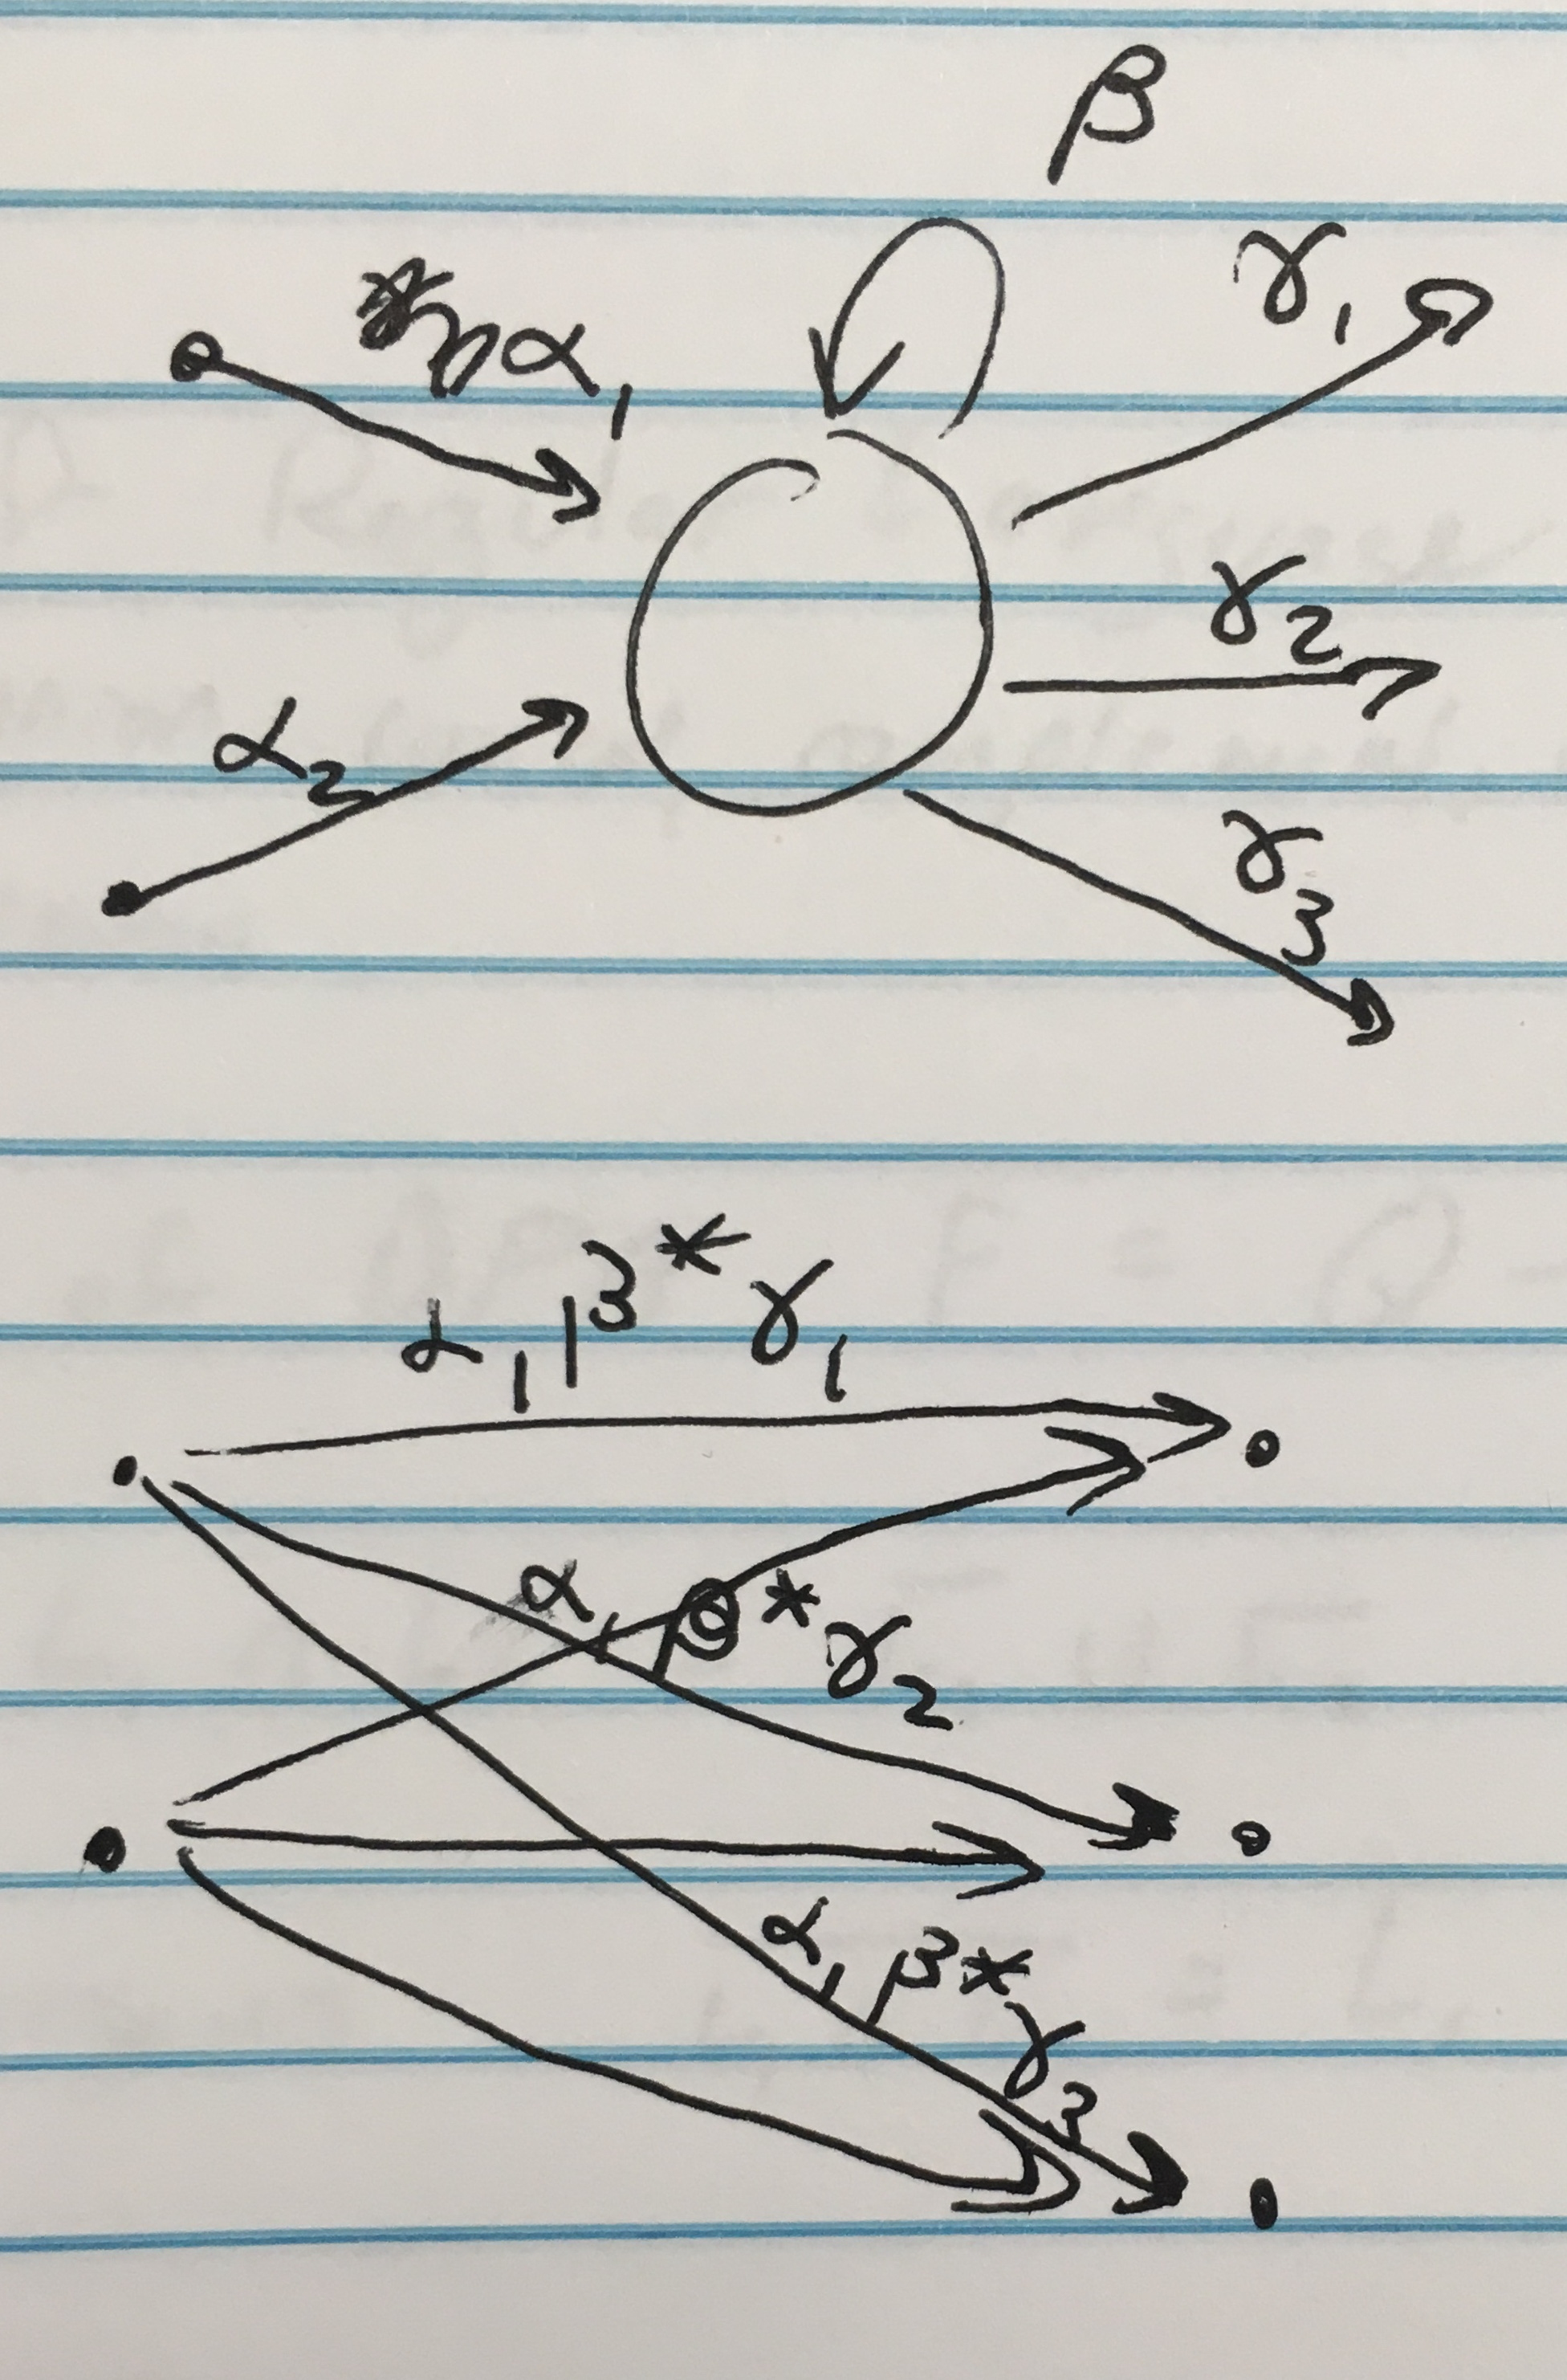
\includegraphics[width=\linewidth]{./figures/f-1.jpg}
   	\end{subfigure}
\end{figure}
\subsection{Simplification of CFG}
Simplification consists of the following steps:
\begin{enumerate}
\item Reduction of CFG
\item Removal of \textbf{Unit Productions}
\item Removal of \textbf{Null Productions}
\end{enumerate}
\subsubsection{Reduction of CFG}
\underline{Phase 1}: Derivation of an equivalent Grammar $G'$, from the CFG G, such that each variable derives some terminal string\\
\underline{Derivation procedure:}
\begin{enumerate}
\item \textbf{Step 1:} Include all symbols $w_1$ that derives some terminal an initialize $i = 1$
\item \textbf{Step 2:} Include symbols $w_{i+1}$ that derives $w_i$
\item \textbf{Step 3:} Increment $i$ and repeat \textbf{Step 2}, until $w_{i+1} = w_i$
\item \textbf{Step 4:} Include all production rules that have $w_i$ in it
\end{enumerate} 
\underline{Phase 2:} Derivation of an equivalent Grammar $G''$, from the CFG, $G'$ such that each symbol appears in a sentential form\\
\underline{Derivation procedure:}
\begin{enumerate}
\item \textbf{Step 1:} Include the Start Symbol in $y_1$ and initialize $i = 1$
\item \textbf{Step 2:} Include all symbols $y_{i+1}$, that can be derived from $y_i$ and include all production rules that have been applied
\item \textbf{Step 3:} Increment $i$ and repeat Step 2, until $y_{i+1} = y_i$
\end{enumerate}
Given below is an example of a CFG with production rules $P$:
\begin{figure}[!htbp]
  	\centering
   	\begin{subfigure}[p]{1.0\linewidth}
    	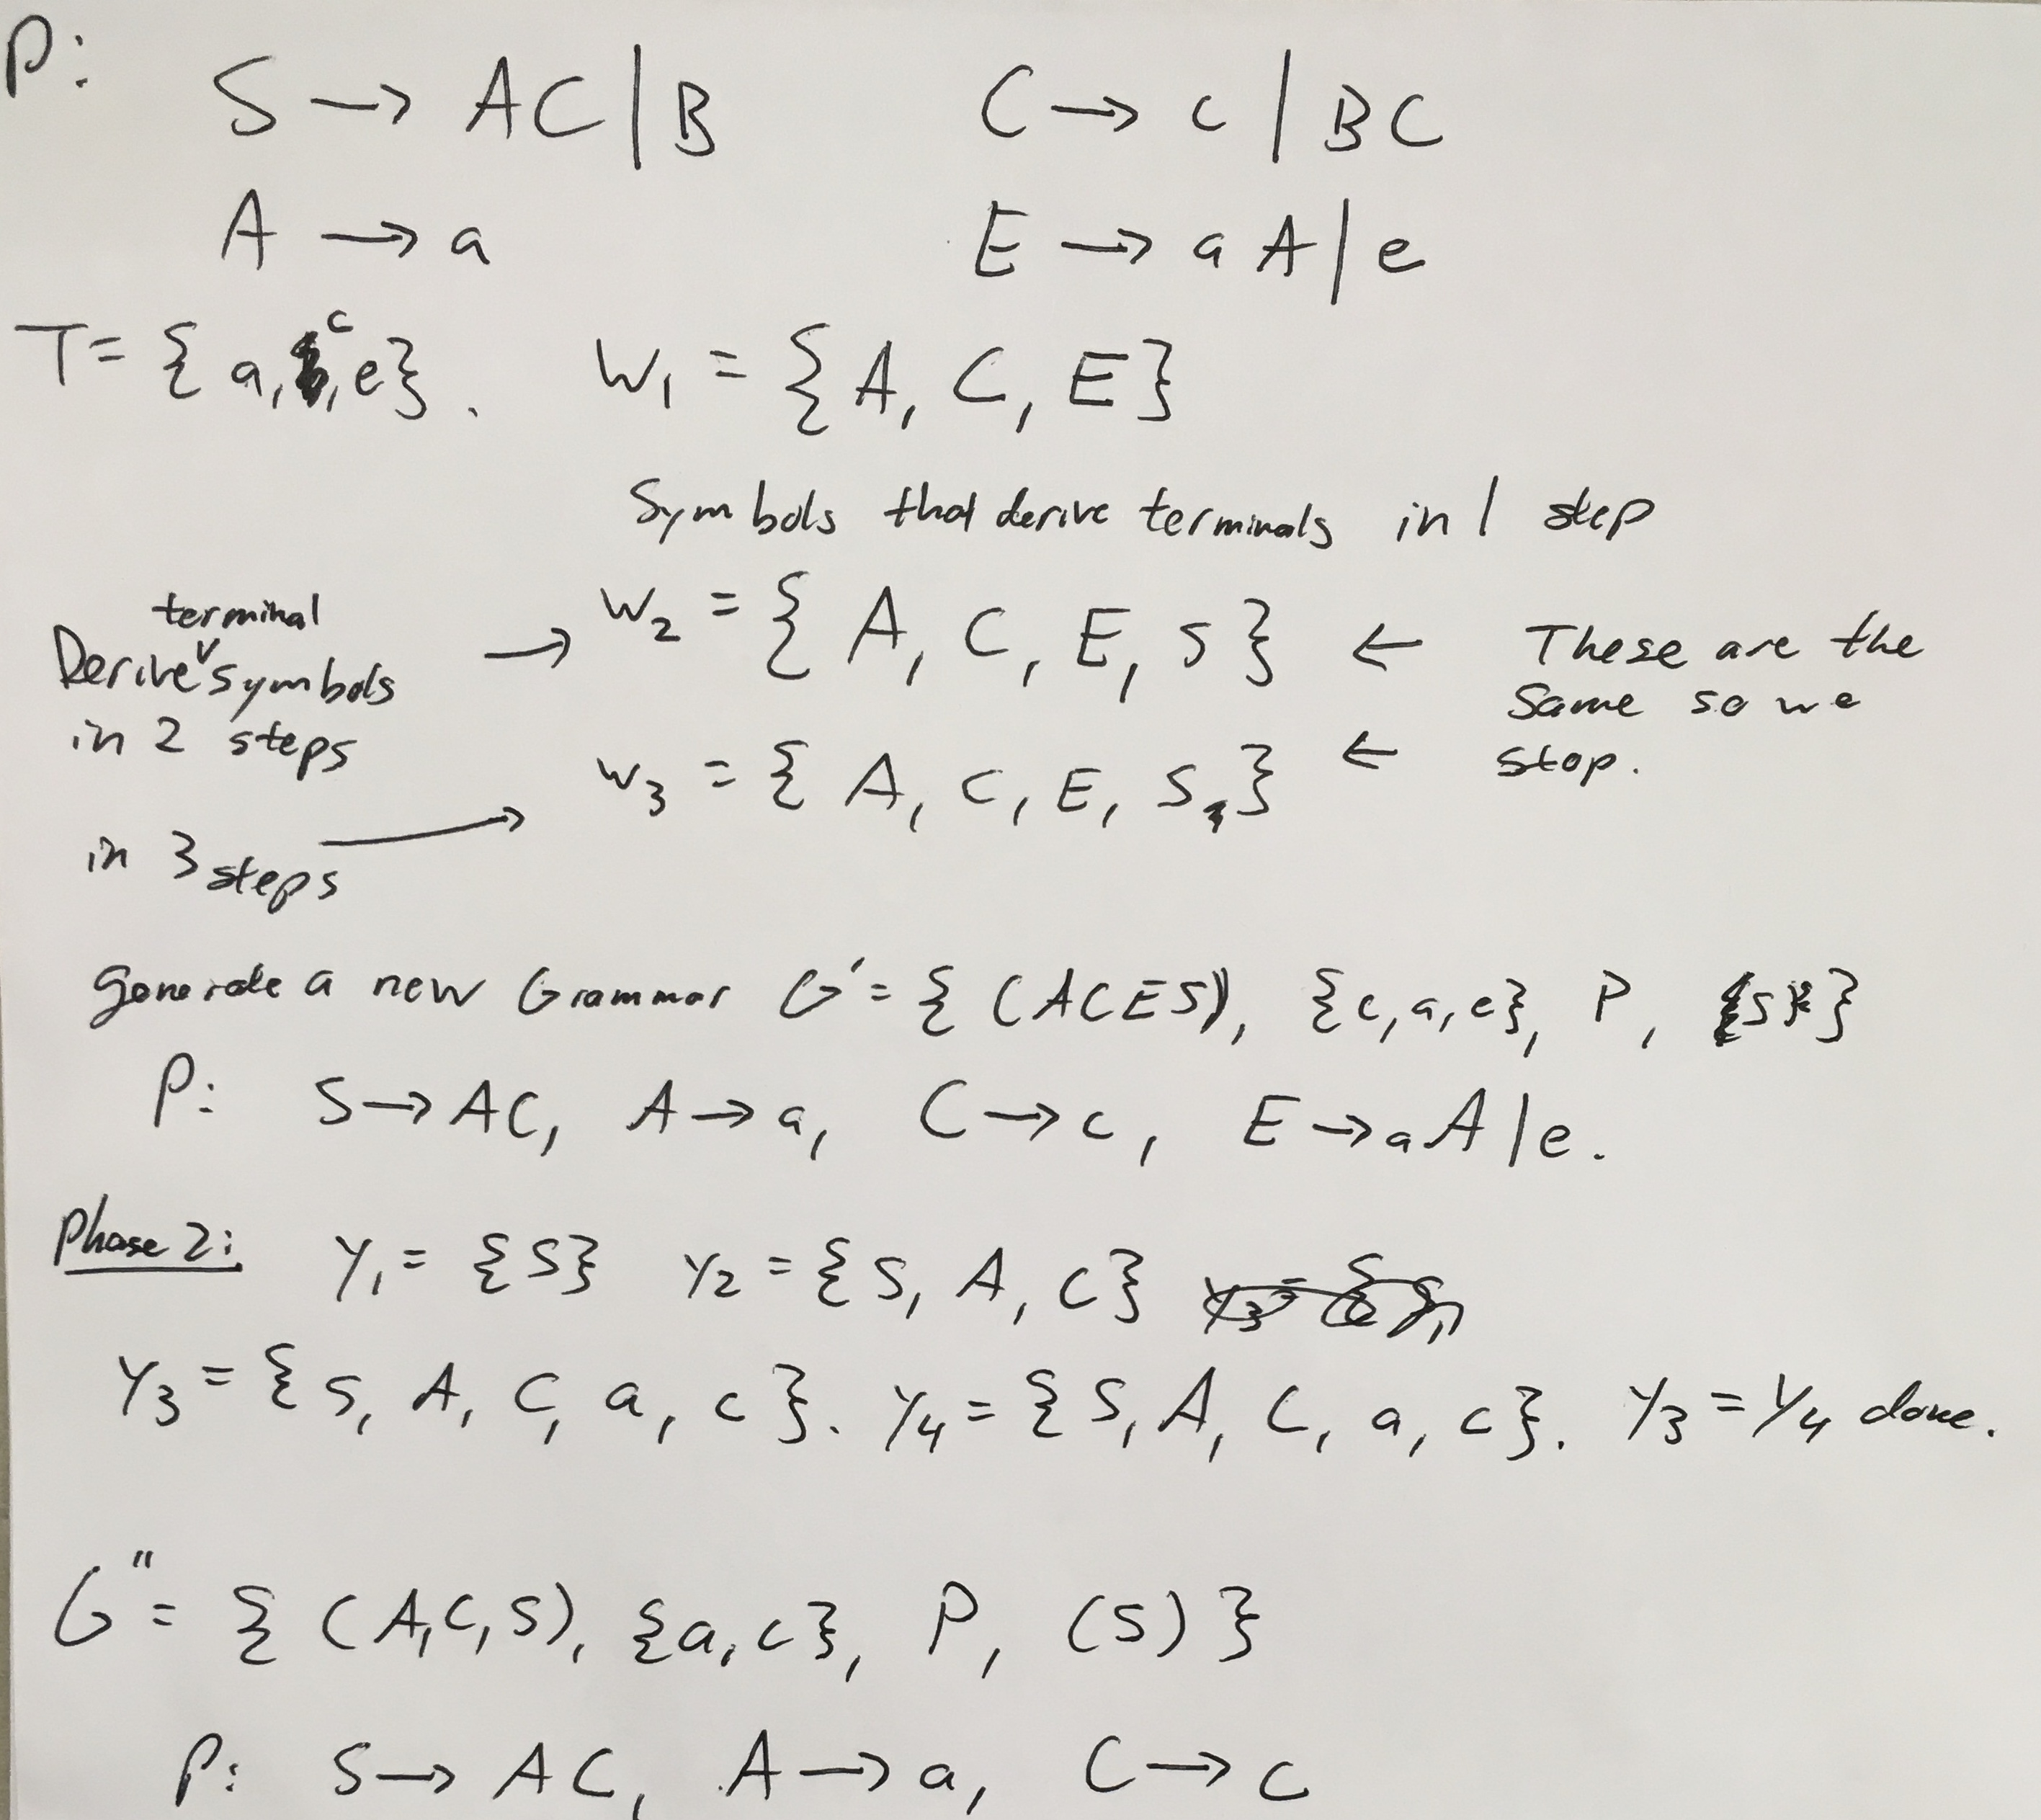
\includegraphics[width=\linewidth]{./figures/f-2.jpg}
   	\end{subfigure}
\end{figure}
\subsubsection{Removal of \textbf{Unit productions}}
Any production rule of the form $A \rightarrow B$, where $A, B \in$ Non Terminals is called a \textbf{Unit Production}\\
\underline{Procedure for removal:}
\begin{enumerate}
\item \textbf{Step 1:} To remove $A\rightarrow B$, add production $A \rightarrow x$ to the grammar rule whenever $B \rightarrow x$ occurs in the grammar. ($x \in $ Terminal, $x$ can be Null)
\item \textbf{Step 2:} Delete $A \rightarrow B$ from the grammar
\item \textbf{Step 3:} Repeat Step 1 until all \textbf{Unit Productions} are removed
\end{enumerate} 
\begin{figure}[!htbp]
  	\centering
   	\begin{subfigure}[p]{1.0\linewidth}
    	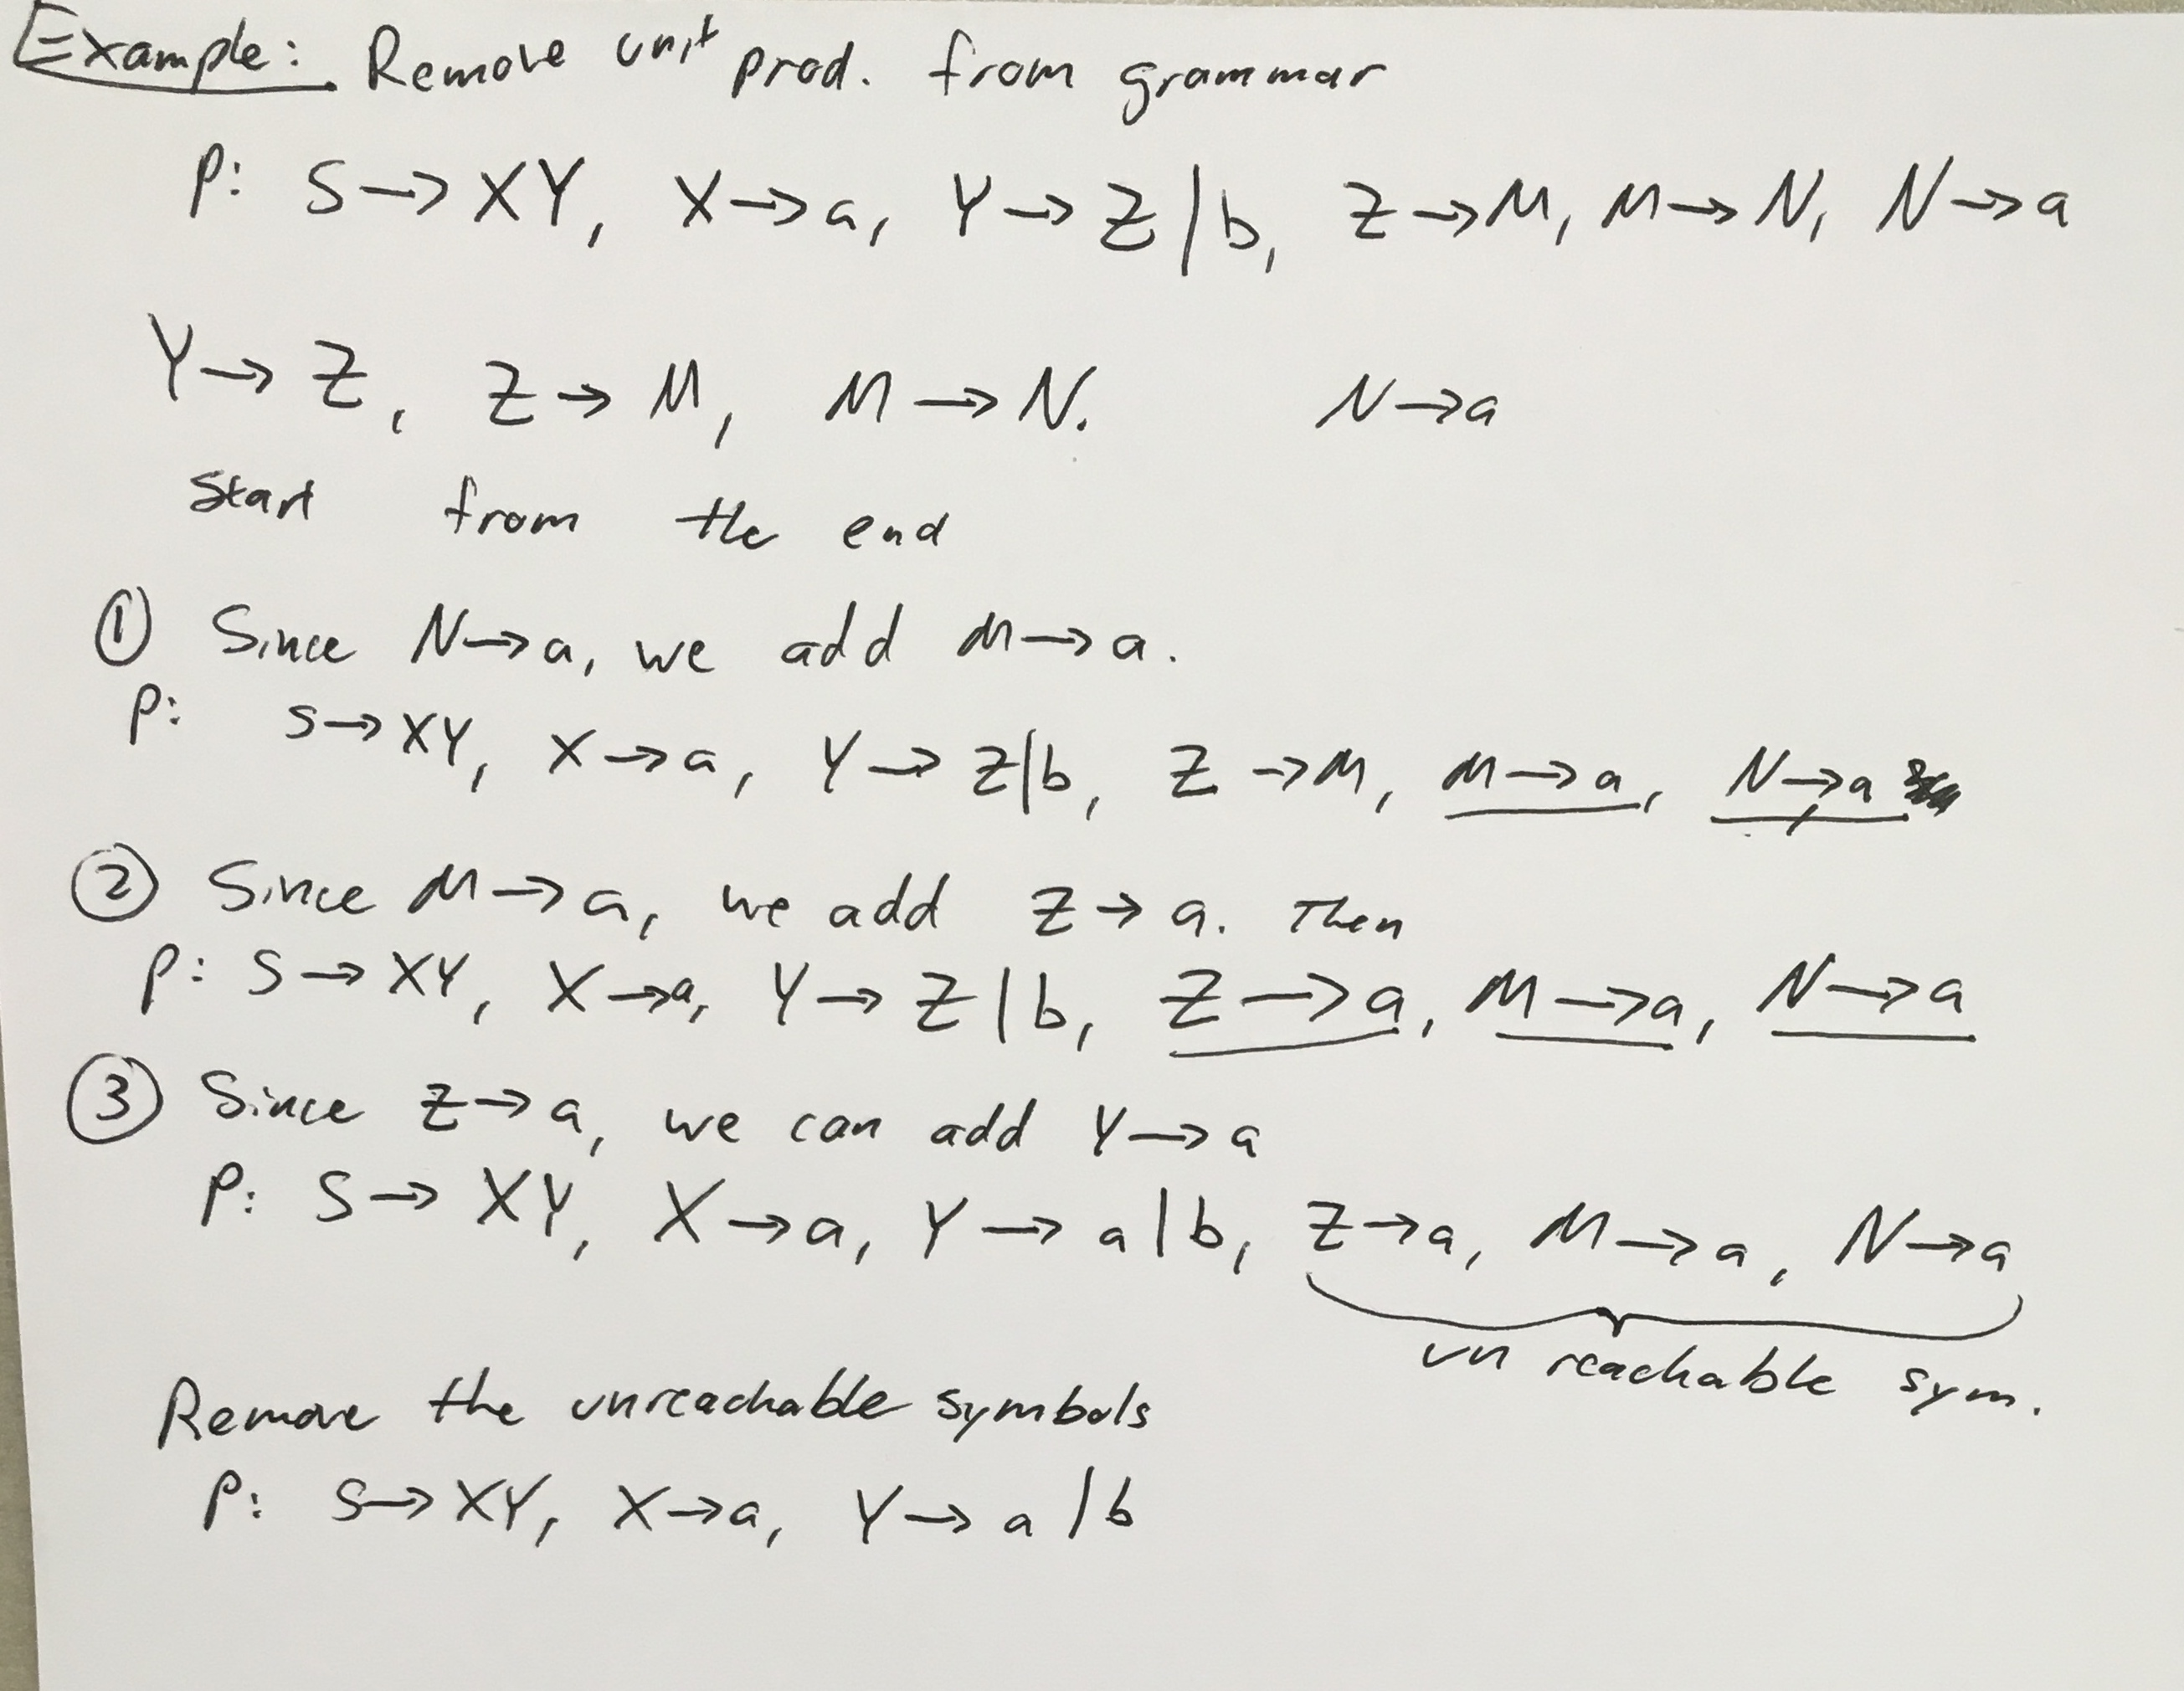
\includegraphics[width=\linewidth]{./figures/f-3.jpg}
   	\end{subfigure}
\end{figure}
\subsubsection{Removal of \textbf{Null Productions}}
In a CFG, a Non-Terminal Symbol $A$ is a nullable variable if there is a production $A \rightarrow \epsilon$ or there is a derivation that starts at $A$ and leads to $\epsilon$ (Like $A \rightarrow^{*} \epsilon$)
\underline{Procedure for removal:}
\begin{enumerate}
\item \textbf{Step 1:} To remove $A \rightarrow \epsilon$, look for all productions whose right side contains $A$
\item \textbf{Step 2:} Replace each occurences of $A$ in each of these productions with $\epsilon$
\item \textbf{Step 3:} Add the resultant productions to the Grammar
\end{enumerate}
\begin{figure}[!htbp]
  	\centering
   	\begin{subfigure}[p]{1.0\linewidth}
    	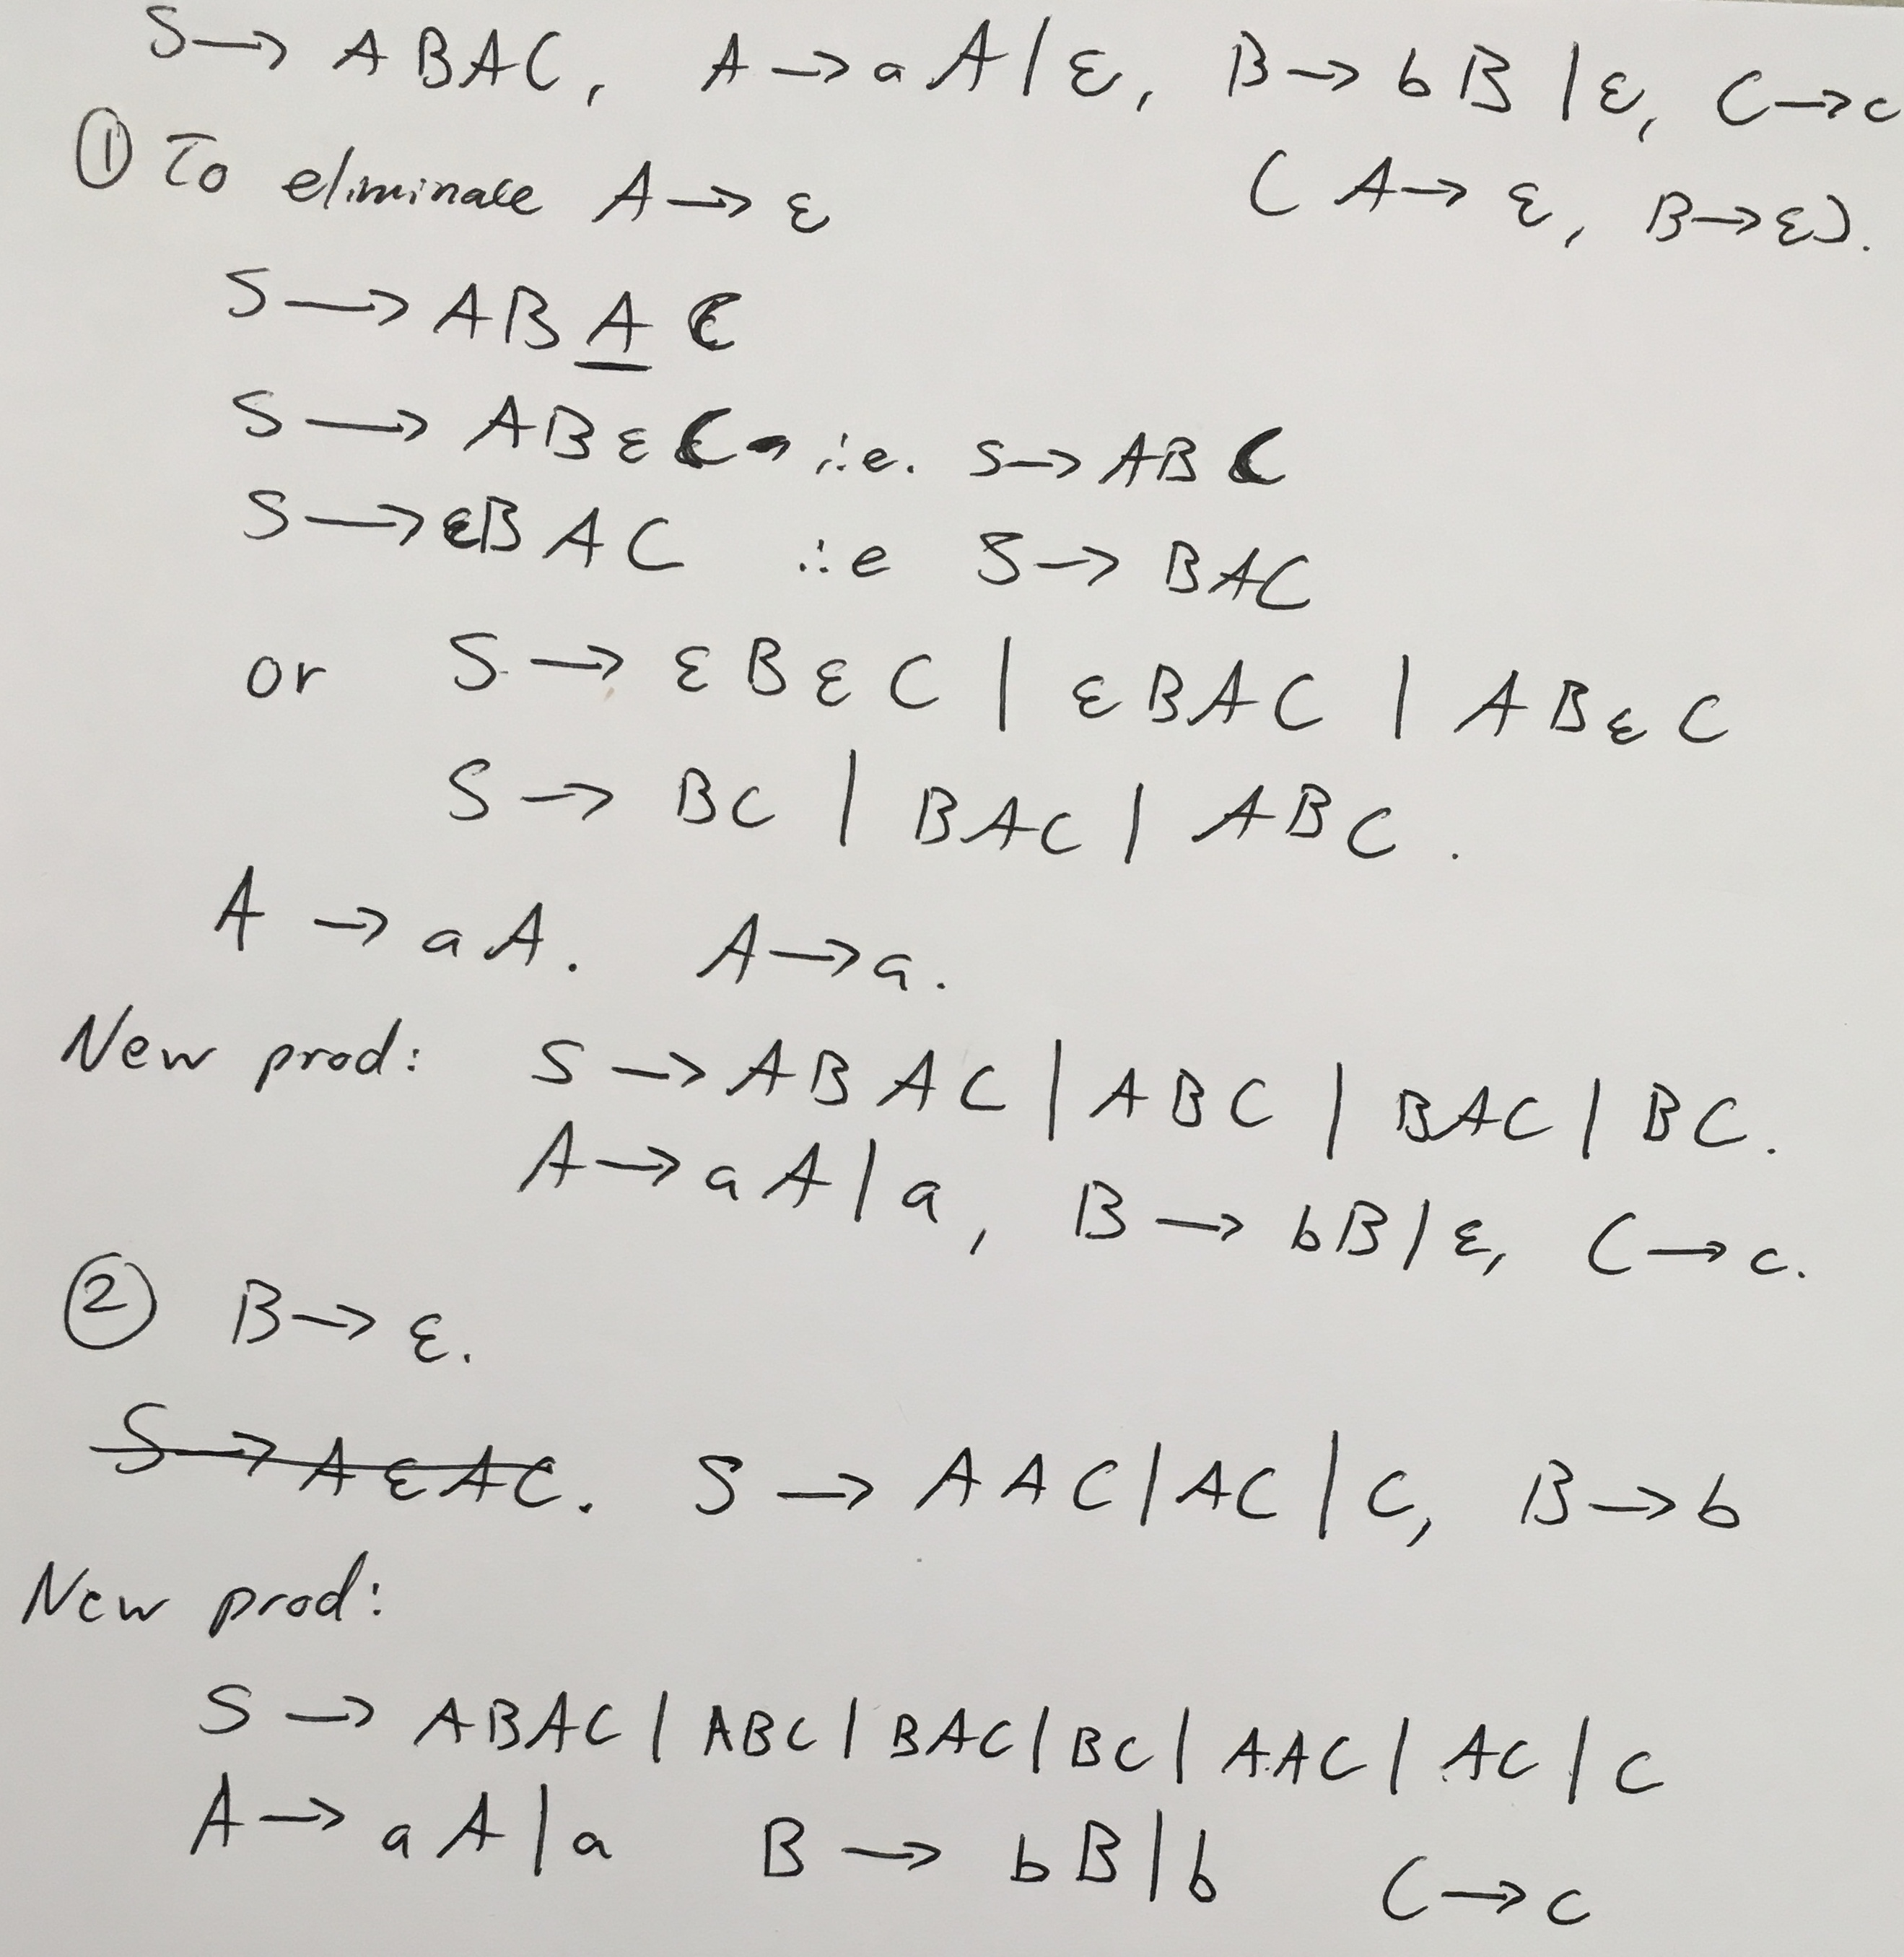
\includegraphics[width=\linewidth]{./figures/f-4.jpg}
   	\end{subfigure}
\end{figure}
\subsubsection{CFG to CNF conversion}
In CNF we have a restriction on the length of the RHS, which is; \textit{elements in RHS should either be \textbf{two variables} or a \textbf{Terminal}}.  A CFG is in CNF if the productions are in the following forms:
\begin{itemize}
\item $A \rightarrow a$
\item $A \rightarrow BC$
\end{itemize}
where $A$, $B$, and $C$ are non-terminals and $a$ is a terminal.\\
\underline{Steps to convert a given CFG to CNF:}
\begin{enumerate}
\item \textbf{Step 1:} If the start symbol $S$ occurs on the RHS, create a new start symbol $S'$ and add a new production rule $S' \rightarrow S$
\item \textbf{Step 2:} Remove Null productions
\item \textbf{Step 3:} Remove Unit productions
\item \textbf{Step 4:} Replace each production $A \rightarrow B_1, ... , B_n$ where $n > 2$ with $A \rightarrow B_1 C$ where $C \rightarrow B_2, ... , B_n$. Repeat this step for all productions having two or more symbols on the right side.
\item \textbf{Step 5:} If the \textbf{RHS} of any production is in the form $A \rightarrow aB$ where $a$ is a terminal and $A$ and $B$ are non-terminals, then the production is replaced by $A \rightarrow XB$ and $X \rightarrow a$.  Repeat this step for every production which is of the form $A \rightarrow aB$.
\end{enumerate}
\end{document}







































